\section{Design}
\label{sec:design}

\subsection{Overview}
\label{sec:overview}

\kunai combines expressive packet filtering with verifier-safe
execution through three components: a protocol-aware filter language,
protocol definitions written in a subset of P4, and verifier-safe code
generation. The filter language describes packet structure and field
conditions, the protocol definitions describe protocol layouts, parser
transitions, and variable-length structures, and the code-generation
stage combines both to produce verifier-accepted eBPF bytecode.
\figref{fig:arch} shows the overall structure.

The compiler takes two inputs, a \kunai filter expression and a set of
protocol definitions written in a subset of P4. It first validates the
layer-chain, resolves field references against the protocol
definitions, and records the information required for later code
generation, rejecting references to non-existent fields, ambiguous
references to repeated protocols, and comparisons whose types do not
match.

The compiler then generates eBPF bytecode that evaluates the filter
condition and returns a match/reject result. A host BPF program
placed at an attach point such as XDP~\cite{hoiland2018xdp},
tc~\cite{tc_man}, or fentry/fexit embeds this bytecode. Under this
split of responsibilities, \kunai handles filter analysis and
bytecode generation, while the host program handles
attach-point-specific context access and follow-on actions such as
capture or drop.

\begin{figure}[t]
  \centering
  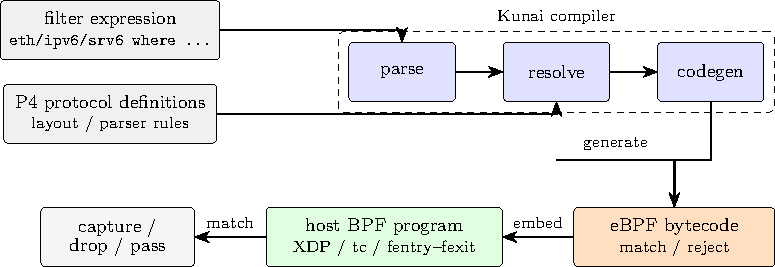
\includegraphics[width=0.8\columnwidth]{figures/fig_arch.pdf}
  \caption{Overview of \kunai.}
  \label{fig:arch}
\end{figure}

\subsection{What the DSL Expresses}
\label{sec:dsl}

The \kunai DSL describes a packet's layer structure and field
conditions as a single filter expression; \figref{fig:grammar} shows
an excerpt of the grammar; the full grammar is available in the
project repository.\footnote{\url{https://github.com/(redacted for review)}}

\begin{figure}[t]
\begin{lstlisting}[basicstyle=\scriptsize\ttfamily,breaklines=true,columns=fullflexible]
filter       ::= layer-chain where-clause?
layer-chain  ::= layer ('/' layer)*
layer        ::= layer-atom quantifier?
layer-atom   ::= proto-name ('@' label)? predicate?
               | '(' layer ('|' layer)+ ')'
quantifier   ::= '?' | '+' | '*' | '{' INT '}' | '{' INT ',' INT '}'
predicate    ::= '[' comparison (',' comparison)* ']'
where-clause ::= 'where' bool-expr
bool-expr    ::= comparison | quant-atom
               | '(' bool-expr ')' | bool-expr bool-op bool-expr
comparison   ::= field-ref op value
quant-atom   ::= ('any' | 'all') '(' bool-expr ')'
field-ref    ::= ident index? ('.' ident index?)*
\end{lstlisting}
\caption{Excerpt of the \kunai filter-expression grammar.}
\label{fig:grammar}
\end{figure}

A layer-chain lists, with \texttt{/}, the order in which protocols
appear in the packet, and can also express optional layers,
repetition, and choice. The \texttt{where} clause is a condition over
the fields of layers in the chain and of auxiliary headers and lists.
\kunai resolves a field reference into one of the forms in
Table~\ref{tab:fieldref}; there, \texttt{<stack>} is not a literal but
the name of an auxiliary header list given in the protocol definition,
such as \texttt{segments} or \texttt{exts}.

\begin{table}[htbp]
  \centering\footnotesize
  \setlength{\tabcolsep}{4pt}
  \begin{tabular}{@{}ll@{}}
    \toprule
    Reference form (example) & Meaning \\
    \midrule
    \texttt{proto.field} (\texttt{tcp.dport}) & primary field of a protocol unique in the chain \\
    \texttt{label.field} (\texttt{inner.dst}) & field of a layer carrying a label (\texttt{@inner}) \\
    \texttt{proto.aux.field} & field of an optional or auxiliary header \\
    \texttt{proto.<stack>[N].field} & static index into an auxiliary header list \\
    \texttt{proto.<stack>.field} & element being walked in \texttt{any()}/\texttt{all()} \\
    \texttt{proto.options.NAME.field} & TCP / IPv4 option lookup \\
    \bottomrule
  \end{tabular}
  \caption{Field-reference forms \kunai resolves.}
  \label{tab:fieldref}
\end{table}

\kunai interprets a field reference inside a bracket predicate as
relative to that layer. In the \texttt{where} clause, references name
the layer explicitly, as in \texttt{proto.field} or
\texttt{label.field}.

When the same protocol appears more than once in a chain,
\texttt{proto.field} alone does not determine which layer to read.
For example, when a chain contains both an outer and an inner IPv4 header,
\texttt{ipv4.dst} does not uniquely identify which destination field
is meant. \kunai rejects such a reference before code generation and
requires a label-qualified reference. A filter on the inner IPv4
destination of a GTP-U tunnel, for example, is written as follows.

\begin{lstlisting}[style=kunai]
eth/ipv4@outer/udp/gtp/ipv4@inner/tcp where inner.dst == 10.0.0.1
\end{lstlisting}

The chain before \texttt{where} lists the layers to traverse, from
Ethernet through an outer IPv4 header, UDP, GTP, an inner IPv4 header,
to TCP, and the \texttt{where} clause gives the field condition checked
once the chain matches, here that the inner IPv4 header's destination
equals \texttt{10.0.0.1}. Here \texttt{@outer} and \texttt{@inner} distinguish the two IPv4
layers. Because \texttt{inner.dst} uniquely names the destination
field of the inner IPv4 header, \kunai can determine which field to read even
though the same \texttt{ipv4} header appears twice.

Variable-length lists are handled with \texttt{any()} and
\texttt{all()}. A filter that matches a packet whose SRv6 segment list
contains a given address, for example, is written as follows.

\begin{lstlisting}[style=kunai]
eth/ipv6/srv6 where any(srv6.segments.addr == fc00::1)
\end{lstlisting}

The scan target of \texttt{any()} and \texttt{all()} is the auxiliary
header list referenced without an index inside the expression, and
there must be exactly one such target list. The same list may be
referenced several times; for example,
\texttt{any(srv6.segments.addr == fc00::1 or srv6.segments.addr ==
fc00::2)} is valid. An \texttt{any()} or \texttt{all()} that references no un-indexed list, or
two different ones, is rejected at the analysis stage rather than
walking one of them. A quantifier that appears to walk two
lists therefore cannot be written. \kunai evaluates the inner condition
against each element of the list. The walk requires a field giving the
element count, the width of each element, a way to advance to the next
element, and a stop condition; the protocol definition supplies these.
TCP options and GTP extension headers are handled the same way when
the protocol definition carries this information.

Through these constructs, the \kunai DSL specifies, within one filter
expression, the order in which headers appear, the disambiguation of
repeated protocols, and the target of a variable-length walk. Code generation
uses this information to translate each field access into an offset
from the layer's start and a bit width.

\subsection{Protocol Definitions via a P4 Subset}
\label{sec:p4subset}

\kunai describes protocol headers and parser rules in a subset of
P4~\cite{p4spec,doenges2021petr4,bosshart2014p4}. Existing P4
descriptions then serve as a reference, and \kunai avoids building the
syntax checker, parser, and tooling that a bespoke protocol-description
language~\cite{mccann2000packettypes,pang2006binpac} would require.

The P4 subset \kunai handles is limited to the parts that describe
header layout and parser transitions. \figref{fig:p4srv6} gives the
SRv6 definition, used by the \texttt{any()} example in \S\ref{sec:dsl}
and filter F8 in \S\ref{sec:eval}.

\begin{figure}[t]
\begin{lstlisting}[basicstyle=\scriptsize\ttfamily,breaklines=true,columns=fullflexible]
// headers, extern ParserCounter, const SRV6_ROUTING_TYPE elided
const bit<8> KUNAI_SRV6_IPV6_NEXT_HEADER = 43;   // IPv6 -> SRv6
parser SRv6Parser(packet_in pkt, out srv6_h hdr,
                  out srv6_seg_h[8] segments) {
  ParserCounter() pc;
  state start {
    pkt.extract(hdr);
    pc.set((bit<8>)(hdr.last_entry + 1));   // segment count
    transition select(hdr.routing_type) {
      SRV6_ROUTING_TYPE: walk;  default: reject; } }
  state walk {
    transition select(pc.is_zero()) { true: accept; false: consume_seg; } }
  state consume_seg {
    pkt.extract(segments.next);   // push one 16-byte segment
    pc.decrement(1);  transition walk; } }
\end{lstlisting}
\caption{SRv6 protocol definition in the \kunai P4 subset.}
\label{fig:p4srv6}
\end{figure}

A definition gives \texttt{header} layouts, a \texttt{transition
select} dispatch such as IPv6 to SRv6 on \texttt{routing\_type}, and a
parser walk over a variable-length list. For SRv6 the
\texttt{ParserCounter} is seeded with \texttt{last\_entry + 1} and one
16-byte segment is extracted per iteration, so the element count and
the \texttt{segments} base follow from the walk itself with no \kunai
annotation, and the array capacity bounds the iteration count for the
verifier. In this way, a protocol definition describes layout,
dispatch, and walk metadata within P4 syntax, and adding one extends
the set of supported protocols without changing the compiler itself.
